\documentclass[12pt]{jreport}
\usepackage{comment}
\usepackage{./sty/eclepsf}
\usepackage{tascmac}
\usepackage{tabularx}
\usepackage{listliketab}
\usepackage[longnamesfirst]{natbib}
\usepackage[dvipdfmx]{graphics}
\usepackage[dvipdfmx]{graphicx}
\usepackage[dvipdfmx]{color}
\usepackage{subfigure}
\usepackage{alltt}
\usepackage{here}
\usepackage{afterpage}
\usepackage{algorithm}
\usepackage{algpseudocode}
\usepackage{./sty/ncodeline}
%\usepackage[dvipdfmx, colorlinks, breaklinks,%
\usepackage[dvipdfmx, breaklinks,%
bookmarks=true, bookmarksnumbered=true,%
bookmarkstype=toc, bookmarksopen=true,bookmarksopenlevel=3,%
pdftitle={RG},%
]{hyperref}
\usepackage{bookmark}

\AtBeginDvi{\special{pdf:tounicode EUC-UCS2}}

\usepackage{fancyhdr}

\usepackage{./sty/doxygenorig}

\usepackage{indentfirst}
\usepackage{url}
\usepackage{listings,./sty/jlisting}

\def\lstlistingname{プログラム}

\lstset{%
 language={C++},
 %backgroundcolor={\color[gray]{.85}},%
 basicstyle={\small\ttfamily},%
 identifierstyle={\small},%
 commentstyle={\small\itshape},%
 keywordstyle={\small\bfseries},%
 ndkeywordstyle={\small\ttfamily},%
 stringstyle={\small\ttfamily},
 frame={tb},
 framesep=1zw,
 breaklines=true,
 numbers=left,%
 xrightmargin=0zw,%
 xleftmargin=1.5zw,%
 numberstyle={\scriptsize},%
 stepnumber=1,
 numbersep=1zw,%
 lineskip=-0.5ex%
}

\usepackage{amssymb}
%\usepackage{supertabular,multirow}

\usepackage{array}
\newcolumntype{M}[1]{>{\centering\arraybackslash}m{#1}}

% A4  size: 297mm*210mm %1pt = 0.35mm
\setlength{\topmargin}{-3.4mm} % 10pt 25.4mm - 3.4mm = 22mm
\setlength{\oddsidemargin}{-0.4mm} % 25.4mm - 0.4mm = 25mm
\setlength{\evensidemargin}{-0.4mm} % 25.4mm - 0.4mm = 25mm
\setlength{\textheight}{231mm} % 660pt % original is 225.75mm 645pt
\setlength{\textwidth}{160mm} % 457pt

\renewcommand{\topfraction}{.99}
\renewcommand{\textfraction}{.0}
\renewcommand{\floatpagefraction}{.99}
\renewcommand{\bibname}{参考文献}


\pagestyle{fancy}
\lhead[]{}

\makeatletter
\def\chaptermark#1{\markboth {\ifnum \c@secnumdepth>\m@ne
\@chapapp\ \thechapter \@chappos\ \fi #1}{}}
\makeatother

% タイトル
\def\title{リズム予測を用いたネットワーク音楽演奏における遅延の影響の軽減手法の提案}
% 英語タイトル
\def\etitle{The Use of Rhythm Prediction to Reduce the Effects of Latency in Network Music Performance}
% 著者(日本語)
\def\author{松藤舜}
% 著者(英語)
\def\eauthor{Shun Matsufuji}
% 学部・研究科
\def\dept{慶應義塾大学 環境情報学部}
% 学部・研究科(英語)
\def\edept{Faculty of Environment and Information Studies, Keio University}

\begin{document}

\pagenumbering{roman}
\begin{titlepage}
  \begin{center}
    \begin{large}
      卒業論文   2023年度(令和05年)\\
      \vspace{24pt}
      \title
      \end{large}
  \end{center}
  \vspace{40em}
  \begin{flushright}
    \large \dept\\
    \author
  \end{flushright}
\end{titlepage}

\thispagestyle{empty}


卒業論文要旨 - 20xx年度 (令和xx年度)
\begin{center}
\begin{large}
\begin{tabular}{|M{0.97\linewidth}|}
    \hline
      \title \\
    \hline
\end{tabular}
\end{large}
\end{center}

~ \\


~ \\
キーワード:\\
\underline{1. 卒業論文},
\underline{2. 村井純研究室},
\underline{3. RG},
\underline{4. LaTeX}
\begin{flushright}
\dept \\
\author
\end{flushright}

\thispagestyle{plain}
\clearpage

Abstract of Bachelor's Thesis - Academic Year 2023
\begin{center}
\begin{large}
\begin{tabular}{|p{0.97\linewidth}|}
    \hline
      \etitle \\
    \hline
\end{tabular}
\end{large}
\end{center}

~ \\

Recently, there has been an ever increasing growing interest in ' Networked Music Performances (NMP)', in which multiple performers perform music in real time over a network.
In NMPs there will always be a delay between the performers, which causes a phase shift in the music performance, causing a breakdown of the performance, which is a fatal problem for NMPs.
However, network delay is unavoidable when assuming a global performance over a network.
In this research, instead of reducing the latency in NMPs, I propose a system that allows performers to play music with each other regardless of the latency.
In doing so, I will discuss the underlying issues of latency in NMPs, introduce past research, and propose a system using music prediction to mitigate the effects of latency.
I have also conducted experiments to show that the proposed system can mitigate the effects of latency even in the presence of latency.

~ \\
Keywords : \\
\underline{1. Network Music Performance},
\underline{2. Latency},
\underline{3. Music Prediction},
\underline{4. OSC}
\begin{flushright}
\edept \\
\eauthor
\end{flushright}

\thispagestyle{plain}
\clearpage

\tableofcontents\thispagestyle{plain} %目次
\clearpage
\listoffigures\thispagestyle{plain} %図目次
\clearpage
\listoftables\thispagestyle{plain} %表目次
\clearpage

\pagenumbering{arabic}
\chapter{序論}
\label{introduction}

本章では本研究の背景,課題及び手法を提示し,本研究の概要を示す.

\section{はじめに}
\label{introduction:background}

\subsection{インターネットを介した音楽演奏への注目}
世界的なインターネット,SNSの普及がもたらしたグローバルなコミュニケーションの発展により,世界中のアーティストをつなぐグローバルな音楽のコミュニティが形成している.
私自身も作曲者,ベース演奏者,DJとして様々な方面でこれらのコミュニティに活発に参加している.

従来まではこのようなインターネットを介したコミュニティでは音楽演奏を共有する手段として,事前に音楽演奏を録音し,ファイル共有サービスなどを用いて音声データを送り合うしかなかった.
バンド,楽団など複数人の同時に合奏を行う音楽形式ではこのような音声データを集めたのち,一人が演奏音声を合成し一つの楽曲として聞ける形に変換するという手段が主流である.


これらの状況を踏まえて今まで以上にインターネットを介した複数の演奏者同士による遠隔にリアルタイムで行う音楽演奏のシステムへの需要が上がっている.
こうした異なる場所にいるミュージシャンをネットワークを介して,同じ部屋にいるのと同じように演奏する音楽演奏を「ネットワーク音楽演奏 (Network Music Performance)\cite{lazzaro}」と呼ぶ.

\subsection{遅延の問題}
ネットワーク音楽演奏において遅延は致命的な問題である.
遅延があると演奏者同士のタイミングがずれ,リズムが崩れてしまう.
相手が演奏している音をリアルタイムで聴き,それに合わせて演奏することが重要な音楽演奏においてはこのような遅延があると演奏は不可能になる.
\cite{latency:effect}などの研究によると100ms以上になると演奏が困難になる.
この遅延の問題を解消するためにYamahaのSyncroom\cite{syncroom}やZoomのS6 SessionTrakなどの遅延を減らすシステムが開発されてきた.
しかし音声のバッファ,演奏者のネット環境,演奏者同士の距離などの様々な原因で遅延が発生してしまうことは避けられない.

その状況を踏まえて本研究ではネットワーク音楽演奏における遅延を減らすのではなく,遅延を前提として演奏に影響を与えないシステムを提案する.

\section{本論文の構成}

本論文における以降の構成は次の通りである.

~\ref{background}章では,背景を述べる.
~\ref{related}章では,本研究における問題提起を述べる.
~\ref{proposed}章では,本研究の提案手法を述べる.
~\ref{implementation}章では,~\ref{proposed}章で述べたシステムの実装について述べる.
~\ref{evaluation}章では,本システムの実験評価を行い,考察する.
~\ref{conclusion}章では,本研究のまとめと今後の課題についてまとめる.


%%% Local Variables:
%%% mode: japanese-latex
%%% TeX-master: "../thesis"
%%% End:

\chapter{背景}
\label{background}

本章では本研究の背景について述べる.

\section{ネットワーク音楽演奏}
ネットワーク音楽演奏で演奏を届ける手法は,VoIPアプリケーションのように音声の波形情報を処理し低遅延で届ける方法\cite{syncroom}\cite{lola}\cite{jacktrip},演奏情報をMIDIを使い楽器,音程,強度などに抽象化し,受信した機器が演奏データを元に音を合成するという方法\cite{rtpmidi}\cite{sourcenode}と,2種類の手法に分けることができる.
本研究では演奏予測を扱いやすい後者の手法をとる.

\section{ネットワーク音楽演奏システムの構造}

\section{演奏情報の表現}
本研究では演奏をMIDIの形式であらわし,演奏情報を伝達する.
MIDIとは

\section{OpenSound Control}
OpenSound Control (OSC)\cite{opensoundcontrol}はソフトやコンピュータ同士でリアルタイムの通信を行うためのプロトコルである.
元々ネットワークを経由した楽器の演奏を前提として開発されているためデータ型としてMIDIを使えるうえ,時刻タグ(OSC Time Tag)をメッセージとまとめて送ることで正確な音の再生のタイミングを送信者から指定することが可能である.
そのうえ,OSCは広く使われていてライブラリや実装が豊富であるため本研究のシステムで採用した.

% GRAPH: OSC BUNDLE AND MESSAGE

OSCのメッセージは単体で,もしくは時刻を指定して同時に再生する複数のメッセージをバンドルにまとめて送ることができる.
32ビットでUNIX時間での秒数を,32ビットで秒数の小数部を表す時刻タグをOSCで使用されるため高解像度で再生の管理が可能であり,時刻タグの精度は本研究では十分とする.


\section{Adaptive Metronome}
BattelloらによるAdaptive Metronome\cite{admet}\cite{admet:experiment}は,演奏者の演奏をリアルタイムで分析し,演奏者の演奏に合わせてメトロノームのテンポを変化させるシステムである.

\begin{figure}[htbp]
  \centering
  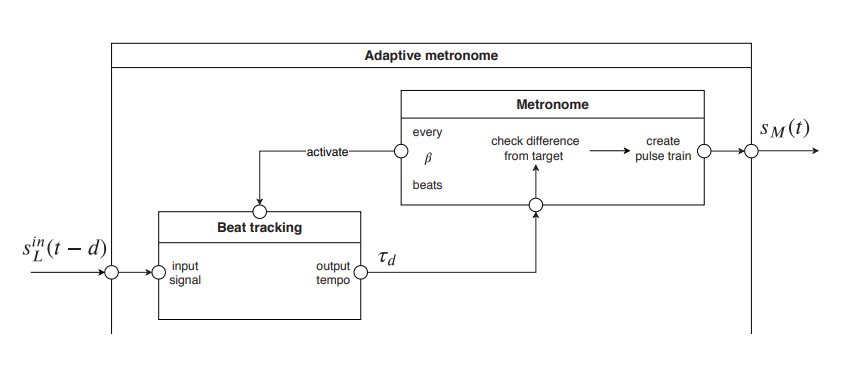
\includegraphics[width=0.8\linewidth]{src/admet.png}
  \caption{Adaptive Metronomeの実験\cite{admet}}
  \label{fig:admet}
\end{figure}

Adaptive Metronomeは親子構造を持っている.
親の演奏者は演奏すると同時にシステムはリアルタイムでその演奏の拍を推定し,子演奏者に音声と拍情報を送信する.
子演奏者のシステムはその情報を受取り,親演奏者の演奏に合わせてメトロノームのテンポを変化させる.
またこのときメトロノームの音は親から子への遅延を考慮して位相をずれして再生される.

こうすることで小演奏者に聞こえるメトロノームは親演奏者の遅延された演奏に関わらず,常に親演奏者の無遅延の演奏に合わせたテンポで再生される.
このシステムを用いた実験では120msの遅延下での演奏を行ったうえでも,被験者は抵抗を感じることなく演奏することができたという結果が得られた.\cite{admet}

\subsection{相互メトロノームの実験}
当初のAdaptive Metronomeの実験では,親演奏者の演奏を子演奏者が聴き,それに合わせて演奏するという形で実験が行われた.
後にBatteloらは親子構造を持たず,相互的にAdaptive Metronomeを聞きあう実験を行った.
実験の結果は現状まだ不十分であるが,このような相互的なシステムでもある程度の効果が得られることが示された.

\subsection{共通テンポの算出}
相互的にAdaptive Metronomeを聞きあう実験では,全体のテンポを決定させる親演奏者がいないため,演奏者同士のテンポと位相が異なる場合がある.
このとき2人の演奏者の状況を踏まえたうえで両方の演奏が同期するような共通のテンポを算出する必要がある.


% 以降は最後にメンション
\section{Tablanet}
Tablanet\cite{tablanet}は,タブラ奏者の演奏をリアルタイムで分析し,演奏者の演奏に合わせてタブラのテンポを変化させるシステムである.

\section{Alexandraki}
Alexandrakiらによる研究\cite{alexandraki:2013}\cite{alexandraki:2014}では,演奏者の演奏をリアルタイムで分析し,事前収録した演奏を実際の演奏に合わせて再生するシステムを提案している.

\chapter{問題提起}
\label{related}

本章では本研究における問題提起について述べる.

\section{ネットワーク音楽演奏における遅延}
遅延はネットワーク音楽演奏のしやすさに大きな影響を与える.
\cite{latency:effect}によると100ms以上の遅延があると演奏者は演奏が困難になる.
これらの遅延の解決を考察するためには,まずネットワーク音楽演奏における遅延を理解する必要がある.

\subsection{遅延のモデル}
この遅延を音楽演奏の文脈でどう捉えられるかを考えるためには,まずモデルを考える必要がある.
\cite{nmp:overview},\cite{latency:model}では音楽演奏は一定の拍を基準として行われているため,音楽演奏者をオシレーターと捉えている.
その場合演奏者による拍を基準とした誤差はオシレーターの周期の位相のずれとして表現できる.
これはすなわち,「演奏の崩れ」と考えることができる.
それを踏まえると,遅延がある中でのネットワーク音楽演奏においての2人の演奏者の関係は,次のような連成振動のモデルで理解することができる.

\begin{figure}
  \centering
  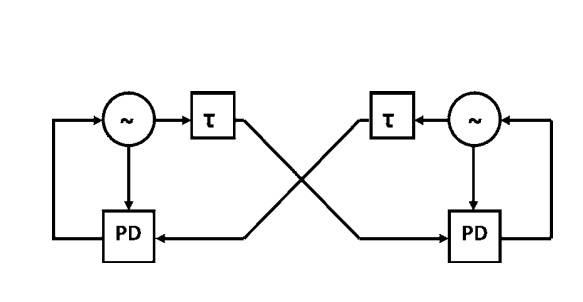
\includegraphics[width=0.8\linewidth]{src/latencymodel.png}
  \caption{連成振動のモデル.\cite{latency:model}より引用}
  \label{fig:oscillator}
\end{figure}

ここでPDはPhase Detector,すなわち演奏者の捉えた拍の感覚,\begin{math}\tau\end{math}は遅延時間である.
このモデルを踏まえて,遅延下の2人の演奏者同士が帰結するテンポは次の式であらわされる.

\begin{displaymath}
  \Omega = \frac{\omega }{1 + K\tau}
\end{displaymath}

\begin{math}\omega \end{math}は両演奏者の平均テンポ,Kは振動の状態更新を表す低数であり,\begin{math}\tau \end{math}は遅延を表す.

\subsection{遅延の原因}
遅延は\ref{background:structure}で述べたすべての工程において発生するが,特に情報の圧縮,ネットワークを介した送信において発生する.

\section{Adaptive Metronomeの問題点}
\label{related:admet}
Adaptive Metronomeは演奏者の演奏をリアルタイムで追跡し,演奏者の演奏に合わせてメトロノームのテンポを変化させるシステムを作ることに成功した.
しかし,このシステムではメトロノームに依存した演奏を行うことになり,特に遅延が大きい場合に各演奏者の演奏相手は相手の演奏者ではなく,メトロノームに必然的になってしまうと考えられる.


%%% Local Variables:
%%% mode: japanese-latex
%%% TeX-master: "./thesis"
%%% End:

\chapter{提案手法}
\label{proposed}

本章では提案手法について述べる.

\section{概要}
本研究では遅延を減らすのではなく,遅延を前提として快適に演奏を行うことができるシステムを目指す.

\section{本システムのアーキテクチャ}
本システムは従来のネットワーク音楽演奏のシステムに加え,拍認識部分,演奏予測,位相修正の3つの部分を追加している.

\begin{figure}[htbp]
  \centering
  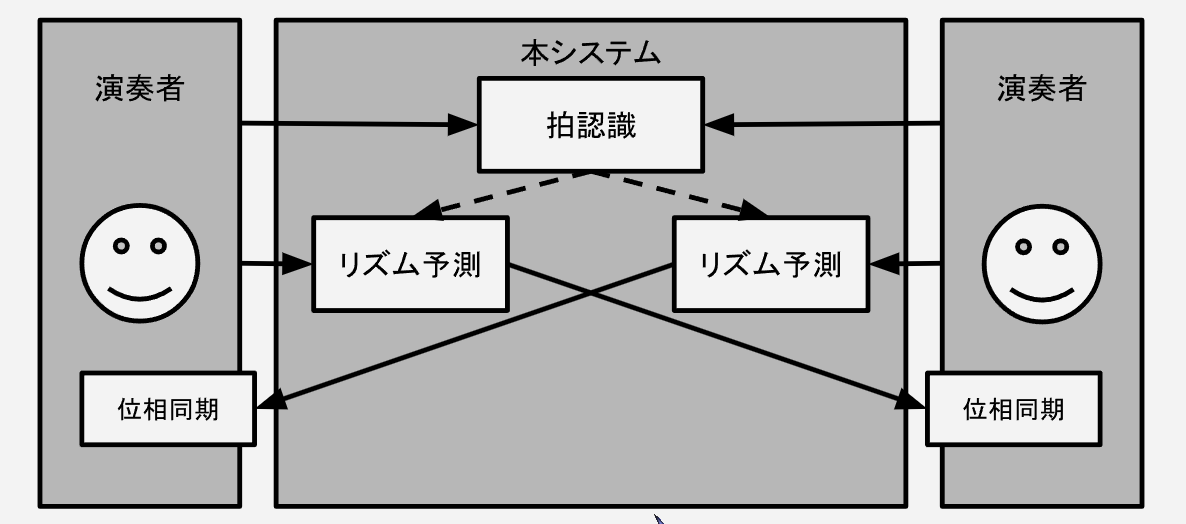
\includegraphics[width=0.8\linewidth]{src/architecture.png}
  \caption{本システムのアーキテクチャ}
  \label{fig:architecture}
\end{figure}

\section{仮説}
遅延のあるネットワーク下でも,演奏相手の演奏を予測しながら演奏を行うことができれば,遅延の量に関係なくまるで同じ部屋にいるかのように演奏できると仮説を立てる.

従来のAdaptive Metronomeと違い,メトロノームの音ではなく予測の音を再生することで演奏者はまるで人間の演奏相手と演奏しているかと同等の体験を得られることができると考える.
本システムを用いると音楽における音のニュアンス,表現を保ちつつ,遅延の補償を行うことができる.
なお音楽的な表現を保つことが目的であるため,表現を伝達するのに十分な予測精度を得られればよいと考える.

%%% Local Variables:
%%% mode: japanese-latex
%%% TeX-master: "../bthesis"
%%% End:

\chapter{実装}
\label{implementation}

本章では提案手法の実装について述べる.

\section{ネットワーク音楽演奏システムのアーキテクチャ}
本システムは従来のネットワーク音楽演奏のシステムに加え,拍認識部分,演奏予測,位相修正の3つの部分を追加している.

\section{演奏予測の実装}
----予測手法について記述

\section{拍認識の実装}
拍認識には様々な手法が存在する.

\section{位相修正}
受信部分において演奏相手の演奏予測を受け取った際,遅延を考慮して位相をずらして再生する必要がある.
これは

%%% Local Variables:
%%% mode: japanese-latex
%%% TeX-master: "../bthesis"
%%% End:

\chapter{実験}
\label{evaluation}
本章では,提案システムの実験評価を行い,考察する.

\section{予測システムの実験}
\subsection{目的}
\subsection{手法}
\subsection{結果}
\subsection{考察}


%%% Local Variables:
%%% mode: japanese-latex
%%% TeX-master: "./thesis"
%%% End:

\chapter{結論}
\label{conclusion}

本章では,本研究のまとめと今後の課題を示す.

\section{本研究のまとめ}

\section{本研究の課題}

\section{今後の展望}

%%% Local Variables:
%%% mode: japanese-latex
%%% TeX-master: "../thesis"
%%% End:

%\appendix
\chapter{付録だよ}


\section{付録内容だよ}

書くよ

\chapter*{謝辞}
\addcontentsline{toc}{chapter}{謝辞}
\label{thanks}

俺に関わった全てに感謝




%%% Local Variables:
%%% mode: japanese-latex
%%% TeX-master: "../yummy_bthesis"
%%% End:


\renewcommand{\thechapter}{\Alph{chapter}}
\setcounter{chapter}{0}
\vspace{-5mm}


\bibliographystyle{unsrt}\pagestyle{plain}
\bibliography{./bib/cites}\pagestyle{plain}
\thispagestyle{plain}%bibtex


\end{document}

%%% Local Variables:
%%% mode: japanese-latex
%%% TeX-master: t
%%% End:
